\documentclass[11pt,a4paper]{article}
\usepackage{amsmath}
\usepackage{geometry}
\usepackage{graphicx}
\usepackage{hyperref}
\usepackage{booktabs}
\usepackage{float}
\usepackage{tikz}
\usepackage{listings}
\usepackage{xcolor}
\usepackage{enumitem}
\usepackage{array}
\usepackage{longtable}
\usepackage{multirow}
\usepackage{fancyhdr}
\usepackage{titlesec}
\usetikzlibrary{arrows.meta, positioning, shapes.geometric, calc, fit,
                backgrounds, decorations.pathreplacing, shapes.symbols}

\geometry{margin=1in, top=1.2in, bottom=1.2in}

% ── Colour palette ────────────────────────────────────────────────────────────
\definecolor{accent}{RGB}{31,111,235}      % blue
\definecolor{accentdark}{RGB}{20,70,160}
\definecolor{okgreen}{RGB}{34,139,34}
\definecolor{warnred}{RGB}{180,30,30}
\definecolor{lightgray}{RGB}{245,245,245}
\definecolor{midgray}{RGB}{200,200,200}
\definecolor{codebg}{RGB}{248,248,248}
\definecolor{codegreen}{RGB}{0,128,0}
\definecolor{codepurple}{RGB}{128,0,128}
\definecolor{codegray}{RGB}{100,100,100}

% ── Code listing style ────────────────────────────────────────────────────────
\lstdefinestyle{zstyle}{
    backgroundcolor=\color{codebg},
    commentstyle=\color{codegreen}\itshape,
    keywordstyle=\color{accent}\bfseries,
    stringstyle=\color{codepurple},
    numberstyle=\tiny\color{codegray},
    basicstyle=\ttfamily\small,
    breaklines=true,
    captionpos=b,
    numbers=left,
    numbersep=6pt,
    frame=single,
    rulecolor=\color{midgray},
    xleftmargin=1.5em,
    framexleftmargin=1.5em,
    showstringspaces=false,
    tabsize=4
}
\lstset{style=zstyle}

% ── Header / footer ───────────────────────────────────────────────────────────
\pagestyle{fancy}
\fancyhf{}
\fancyhead[L]{\small\textcolor{accentdark}{\textbf{HDV Simulator — Security Hardening}}}
\fancyhead[R]{\small\textcolor{codegray}{STM32H753ZI / Zephyr RTOS 3.7}}
\fancyfoot[C]{\small\thepage}
\renewcommand{\headrulewidth}{0.4pt}

% ── Section title styling ─────────────────────────────────────────────────────
\titleformat{\section}{\large\bfseries\color{accentdark}}{}{0em}{}[\color{midgray}\titlerule]
\titleformat{\subsection}{\normalsize\bfseries\color{accent}}{}{0em}{}

% ── TikZ node styles ──────────────────────────────────────────────────────────
\tikzset{
  block/.style={rectangle, rounded corners=4pt, draw=accent, fill=lightgray,
                text width=4.2cm, align=center, minimum height=1cm,
                font=\small},
  decision/.style={diamond, draw=accentdark, fill=lightgray!60,
                   text width=2.8cm, align=center, aspect=1.8,
                   font=\small},
  term/.style={rectangle, rounded corners=8pt, draw=accentdark,
               fill=accentdark!15, text width=3.5cm, align=center,
               minimum height=0.9cm, font=\small\bfseries},
  okblock/.style={block, draw=okgreen, fill=okgreen!10},
  errblock/.style={block, draw=warnred, fill=warnred!10},
  arr/.style={-{Stealth[length=6pt]}, thick, color=accentdark},
}

\hypersetup{
    colorlinks=true, linkcolor=accentdark,
    urlcolor=accent, citecolor=accentdark,
    pdftitle={HDV Simulator Security Hardening},
    pdfauthor={mtilocca}
}

% ─────────────────────────────────────────────────────────────────────────────
\begin{document}

\begin{titlepage}
\centering
\vspace*{2cm}
{\Huge\bfseries\color{accentdark} Security Hardening\\[0.4em]
\large Heavy-Duty Electric Vehicle Simulator}\\[1.5em]
\textcolor{codegray}{\rule{0.6\textwidth}{0.6pt}}\\[1em]
{\large STM32H753ZI \enspace$\cdot$\enspace Nucleo-H753ZI \enspace$\cdot$\enspace Zephyr RTOS 3.7}\\[0.5em]
{\large MCUboot 2.x \enspace$\cdot$\enspace ECDSA-P256 \enspace$\cdot$\enspace OTA via HTTP}\\[2em]
\begin{tabular}{ll}
\textbf{Author}  & mtilocca \\
\textbf{Date}    & April 2026 \\
\textbf{Phases}  & 1 (HTTP Auth) \enspace 2 (IWDG) \enspace 3a (MCUboot) \enspace 3b (OTA) \\
\textbf{Status}  & Phases 1--3b complete; Phase 4 (RDP) deferred to production \\
\end{tabular}
\vfill
\textcolor{codegray}{\small This document covers the security architecture, implementation decisions,\\
flash layout, key management, and threat model for the embedded simulator.}
\end{titlepage}

\tableofcontents
\newpage

% ═════════════════════════════════════════════════════════════════════════════
\section{Overview}

The simulator runs on an STM32H753ZI microcontroller (Cortex-M7, 480 MHz, 2~MB flash, 1~MB RAM)
connected via Ethernet to a LAN. Security was added in four independent layers so that no single
failure collapses all protections.

\begin{center}
\begin{tabular}{@{}clll@{}}
\toprule
\textbf{Phase} & \textbf{Control} & \textbf{Primary Threat Addressed} & \textbf{Status} \\
\midrule
1 & HTTP Bearer token + session cookie & Unauthenticated HTTP commands & \textcolor{okgreen}{\checkmark} \\
2 & IWDG hardware watchdog             & Firmware hang / DoS            & \textcolor{okgreen}{\checkmark} \\
3a & MCUboot ECDSA-P256 signature      & Unsigned firmware execution    & \textcolor{okgreen}{\checkmark} \\
3b & Authenticated OTA endpoint        & Unauthenticated firmware update & \textcolor{okgreen}{\checkmark} \\
4  & RDP Level 1 option bytes          & Flash readback / extraction    & Deferred \\
\bottomrule
\end{tabular}
\end{center}

% ═════════════════════════════════════════════════════════════════════════════
\section{Phase 1 — HTTP Authentication}

\subsection{Token Architecture}

A 64-character hexadecimal Bearer token (256 bits of entropy) is generated once at deployment
by \texttt{scripts/gen\_http\_token.sh} and stored in \texttt{http\_auth.hpp} (gitignored).
The token never changes between reboots; it is the shared secret between the operator and the board.

Browser sessions are managed separately: a successful \texttt{POST /login} with the correct token
creates a 32-character random hex session token stored in an on-device table of four slots
with a one-hour TTL.

\subsection{Authentication Flow}

\begin{center}
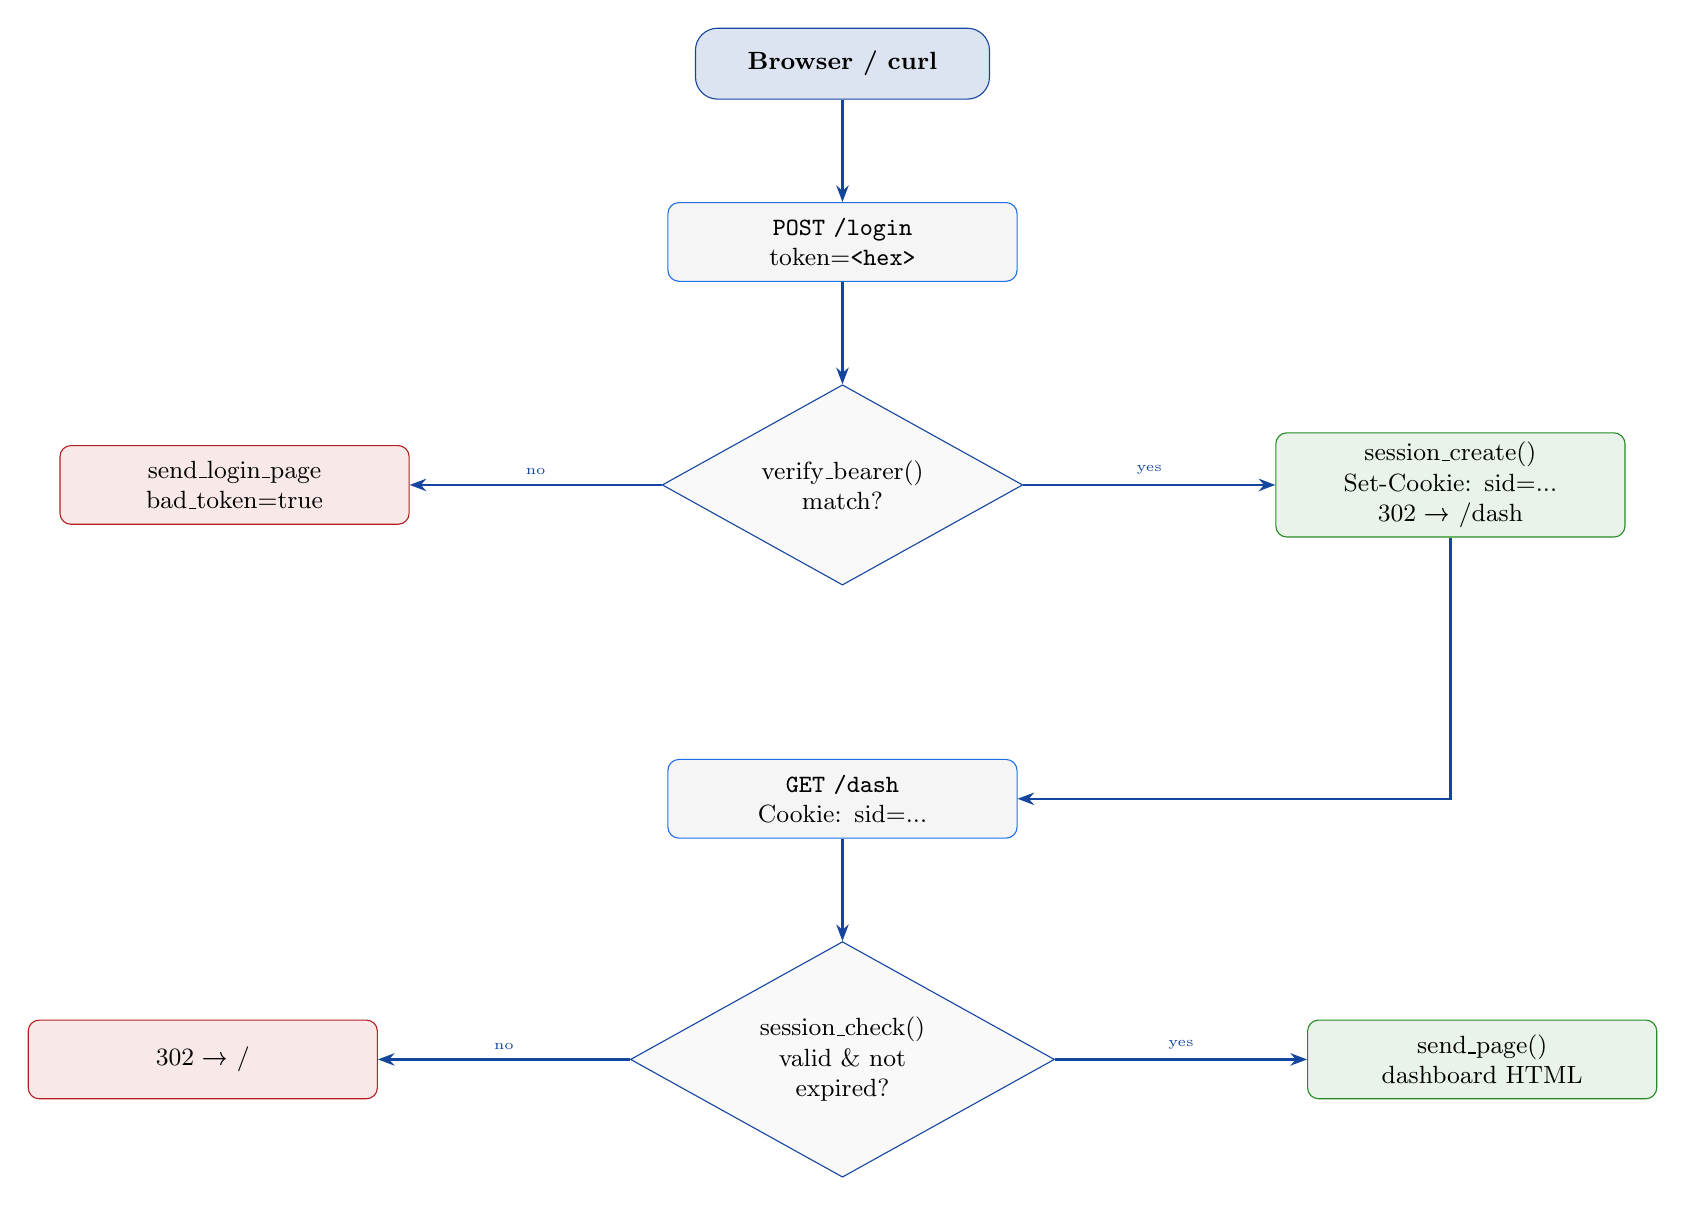
\begin{tikzpicture}[node distance=1.3cm, every node/.style={font=\small}]
  \node[term]                    (start) {Browser / curl};
  \node[block, below=of start]   (req)   {\texttt{POST /login}\\token=\texttt{<hex>}};
  \node[decision, below=of req]  (vfy)   {verify\_bearer()\\match?};
  \node[okblock, right=3.2cm of vfy] (ok)  {session\_create()\\Set-Cookie: sid=...\\302 → /dash};
  \node[errblock, left=3.2cm of vfy] (bad) {send\_login\_page\\bad\_token=true};
  \node[block, below=2.2cm of vfy] (dash) {\texttt{GET /dash}\\Cookie: sid=...};
  \node[decision, below=of dash]  (ses)  {session\_check()\\valid \& not expired?};
  \node[okblock, right=3.2cm of ses] (page) {send\_page()\\dashboard HTML};
  \node[errblock, left=3.2cm of ses] (redir){302 → /};

  \draw[arr] (start) -- (req);
  \draw[arr] (req)   -- (vfy);
  \draw[arr] (vfy)   -- node[above,font=\tiny]{yes} (ok);
  \draw[arr] (vfy)   -- node[above,font=\tiny]{no}  (bad);
  \draw[arr] (ok)    |- (dash);
  \draw[arr] (dash)  -- (ses);
  \draw[arr] (ses)   -- node[above,font=\tiny]{yes} (page);
  \draw[arr] (ses)   -- node[above,font=\tiny]{no}  (redir);
\end{tikzpicture}
\end{center}

\subsection{Residual Risk}

Without TLS, the Bearer token and session cookie are transmitted in plaintext over the LAN.
A passive observer on the same subnet can capture and replay the token.
This is mitigated in the current deployment by a physically isolated LAN; HTTPS will
be added in the next phase to eliminate this residual risk.

% ═════════════════════════════════════════════════════════════════════════════
\section{Phase 2 — IWDG Hardware Watchdog}

\subsection{Configuration}

\begin{center}
\begin{tabular}{@{}ll@{}}
\toprule
\textbf{Parameter} & \textbf{Value} \\
\midrule
Clock source       & LSI (32 kHz, independent of main PLL) \\
Prescaler (PR)     & 6 → divide-by-256 → 125 Hz tick \\
Reload (RLR)       & 624 → timeout = 625/125 = \textbf{5.0 s} \\
Zephyr API timeout & 1~s (\texttt{wdt\_install\_timeout}, \texttt{window.max=1000}) \\
Grace period       & 10~s (watchdog thread feeds every 500~ms while threads start) \\
Monitoring         & \texttt{k\_sem\_take(g\_wdt\_sem, K\_MSEC(500))} — given by plant\_thread \\
\bottomrule
\end{tabular}
\end{center}

\subsection{Early Boot Kick Sequence}

The IWDG cannot be stopped once started and persists across warm resets.
Before the Zephyr thread scheduler starts, the watchdog timer could expire if it was inherited
from a previous session. Four \texttt{SYS\_INIT\_NAMED} hooks write \texttt{0xAAAA} directly
to the IWDG1 key register (hardware kick, no driver needed):

\begin{lstlisting}[language=C, caption={Early IWDG kicks in watchdog\_thread.cpp}]
static volatile uint32_t* const IWDG1_KR = (volatile uint32_t*)0x58004800U;

static int iwdg_early_kick(void) { *IWDG1_KR = 0xAAAAU; return 0; }

SYS_INIT_NAMED(iwdg_kick_pk1, iwdg_early_kick, PRE_KERNEL_1, 0);
SYS_INIT_NAMED(iwdg_kick_pk2, iwdg_early_kick, PRE_KERNEL_2, 0);
SYS_INIT_NAMED(iwdg_kick_pok, iwdg_early_kick, POST_KERNEL,  0);
SYS_INIT_NAMED(iwdg_kick_app, iwdg_early_kick, APPLICATION,  0);
\end{lstlisting}

\subsection{Boot-Loop Root Cause (Postmortem)}

During Phase~2 integration the board entered a hard reset loop at 52~ms post-power-on.
Root cause: the IWDG was inherited from a prior session with a short timeout and no early
kick was issued. The fix above — direct register writes at every SYS\_INIT level — ensures
the counter is reset before any of the four boot phases can exhaust it.
Full postmortem: \texttt{docs/zephyr/IWDG\_BOOT\_LOOP\_POSTMORTEM.md}.

% ═════════════════════════════════════════════════════════════════════════════
\section{Phase 3a — MCUboot Secure Bootloader}

\subsection{Flash Partition Layout}

The STM32H753ZI has 2~MB dual-bank flash with 128~KB sectors.
The board default partitions were overridden in both \texttt{app.overlay}
and \texttt{sysbuild/mcuboot.overlay}.

\begin{center}
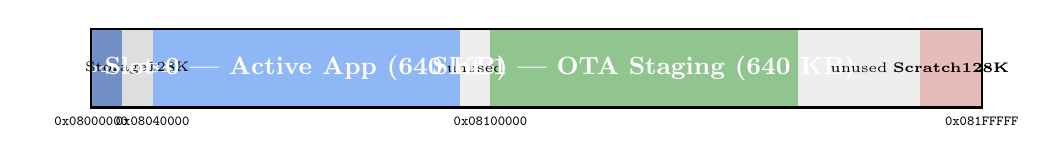
\begin{tikzpicture}[font=\small]
  % Flash bar
  \def\W{10}   % total width in cm
  % Sections: boot=0.5, storage=0.5, slot0=2.5, unused=0.5, slot1=2.5, unused=1, scratch=0.5 → total=8
  \def\scale{0.39}  % scale factor: 128KB → 0.5cm

  % Draw blocks
  \fill[accentdark!60] (0,0) rectangle (0.5*\scale*2,1);      % boot 128KB
  \fill[midgray!60]    (0.5*\scale*2,0) rectangle (1*\scale*2,1);  % storage 128KB
  \fill[accent!50]     (1*\scale*2,0) rectangle (6*\scale*2,1);    % slot0 640KB
  \fill[midgray!30]    (6*\scale*2,0) rectangle (6.5*\scale*2,1);  % unused 128KB
  \fill[okgreen!50]    (6.5*\scale*2,0) rectangle (11.5*\scale*2,1); % slot1 640KB
  \fill[midgray!30]    (11.5*\scale*2,0) rectangle (13.5*\scale*2,1);% unused 256KB
  \fill[warnred!30]    (13.5*\scale*2,0) rectangle (14.5*\scale*2,1);% scratch 128KB

  % Labels inside
  \node[font=\tiny\bfseries,color=white] at (0.25*\scale*2, 0.5) {MCUboot\\128K};
  \node[font=\tiny,color=black]          at (0.75*\scale*2, 0.5) {Storage\\128K};
  \node[font=\small\bfseries,color=white] at (3.5*\scale*2, 0.5) {Slot 0 — Active App (640 KB)};
  \node[font=\tiny,color=black]           at (6.25*\scale*2,0.5) {\tiny unused};
  \node[font=\small\bfseries,color=white] at (9*\scale*2,  0.5)  {Slot 1 — OTA Staging (640 KB)};
  \node[font=\tiny,color=black]           at (12.5*\scale*2,0.5) {\tiny unused};
  \node[font=\tiny\bfseries,color=black]  at (14*\scale*2, 0.5)  {Scratch\\128K};

  % Border
  \draw[thick] (0,0) rectangle (14.5*\scale*2,1);

  % Address labels below
  \node[font=\tiny,below] at (0,0)             {\texttt{0x08000000}};
  \node[font=\tiny,below] at (1*\scale*2,0)    {\texttt{0x08040000}};
  \node[font=\tiny,below] at (6.5*\scale*2,0)  {\texttt{0x08100000}};
  \node[font=\tiny,below] at (14.5*\scale*2,0) {\texttt{0x081FFFFF}};
\end{tikzpicture}
\end{center}

\begin{center}
\begin{tabular}{@{}lllll@{}}
\toprule
\textbf{Partition} & \textbf{Address} & \textbf{Size} & \textbf{Sectors} & \textbf{Purpose} \\
\midrule
\texttt{boot\_partition}    & \texttt{0x08000000} & 128 KB & Bank1 S0     & MCUboot bootloader \\
\texttt{storage\_partition} & \texttt{0x08020000} & 128 KB & Bank1 S1     & Board default, unused \\
\texttt{slot0\_partition}   & \texttt{0x08040000} & 640 KB & Bank1 S2--6  & Active application \\
(unused)                    & \texttt{0x080E0000} & 128 KB & Bank1 S7     & Reserved \\
\texttt{slot1\_partition}   & \texttt{0x08100000} & 640 KB & Bank2 S0--4  & OTA staging \\
(unused)                    & \texttt{0x081A0000} & 256 KB & Bank2 S5--6  & Reserved \\
\texttt{scratch\_partition} & \texttt{0x081E0000} & 128 KB & Bank2 S7     & MCUboot scratch \\
\bottomrule
\end{tabular}
\end{center}

\subsection{Boot Verification Flow}

\begin{center}
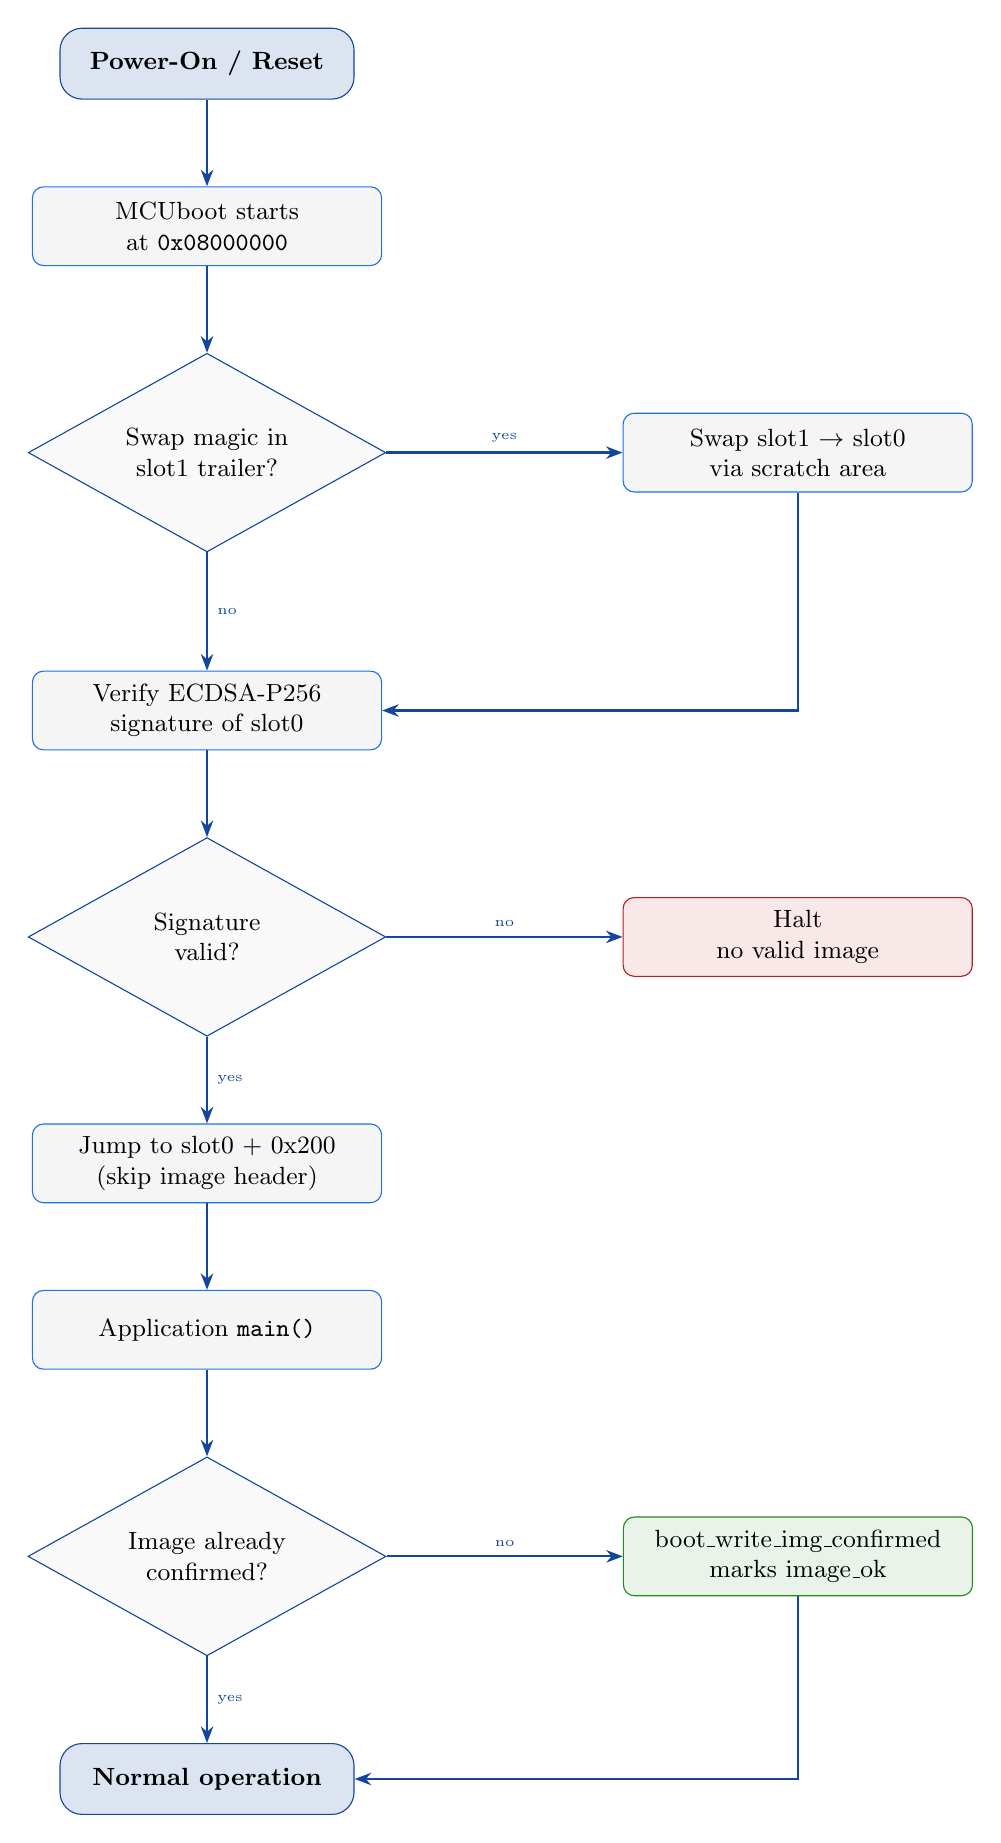
\begin{tikzpicture}[node distance=1.1cm, every node/.style={font=\small}]
  \node[term]                      (rst)  {Power-On / Reset};
  \node[block, below=of rst]       (mb)   {MCUboot starts\\at \texttt{0x08000000}};
  \node[decision, below=of mb]     (swp)  {Swap magic in\\slot1 trailer?};
  \node[block, right=3cm of swp]   (do_swap) {Swap slot1 $\to$ slot0\\via scratch area};
  \node[block, below=1.5cm of swp] (vfy)  {Verify ECDSA-P256\\signature of slot0};
  \node[decision, below=of vfy]    (sig)  {Signature\\valid?};
  \node[errblock, right=3cm of sig](halt) {Halt\\no valid image};
  \node[block, below=of sig]       (jmp)  {Jump to slot0 + 0x200\\(skip image header)};
  \node[block, below=of jmp]       (app)  {Application \texttt{main()}};
  \node[decision, below=of app]    (cnf)  {Image already\\confirmed?};
  \node[okblock, right=3cm of cnf] (wrt)  {boot\_write\_img\_confirmed\\marks image\_ok};
  \node[term, below=of cnf]        (run)  {Normal operation};

  \draw[arr] (rst)  -- (mb);
  \draw[arr] (mb)   -- (swp);
  \draw[arr] (swp)  -- node[above,font=\tiny]{yes} (do_swap);
  \draw[arr] (do_swap) |- (vfy);
  \draw[arr] (swp)  -- node[right,font=\tiny]{no} (vfy);
  \draw[arr] (vfy)  -- (sig);
  \draw[arr] (sig)  -- node[above,font=\tiny]{no}  (halt);
  \draw[arr] (sig)  -- node[right,font=\tiny]{yes} (jmp);
  \draw[arr] (jmp)  -- (app);
  \draw[arr] (app)  -- (cnf);
  \draw[arr] (cnf)  -- node[above,font=\tiny]{no}  (wrt);
  \draw[arr] (wrt)  |- (run);
  \draw[arr] (cnf)  -- node[right,font=\tiny]{yes} (run);
\end{tikzpicture}
\end{center}

\subsection{Signing Key Management}

\begin{center}
\begin{tabular}{@{}lll@{}}
\toprule
\textbf{Artefact} & \textbf{Location} & \textbf{Notes} \\
\midrule
Private key (\texttt{mcuboot\_signing\_key.pem}) & \texttt{zephyr/} & ECDSA-P256; gitignored; generated once \\
Public key & Embedded in MCUboot binary & Derived from private key at build time \\
Signed app (\texttt{zephyr.signed.bin}) & Build output & Signed by \texttt{imgtool} during \texttt{west build} \\
\bottomrule
\end{tabular}
\end{center}

Generate the signing key (run once):
\begin{lstlisting}[language=bash]
python3 /path/to/mcuboot/scripts/imgtool.py keygen \
    -k zephyr/mcuboot_signing_key.pem -t ecdsa-p256
\end{lstlisting}

The public key is embedded in MCUboot at compile time via \texttt{MCUBOOT\_SIGNING\_KEY\_FILE}
in \texttt{CMakeLists.txt}. The private key must be available at every build that produces a
firmware image; it is never stored on the device.

\subsection{Image Format}

Each signed binary has the following structure in flash:

\begin{center}
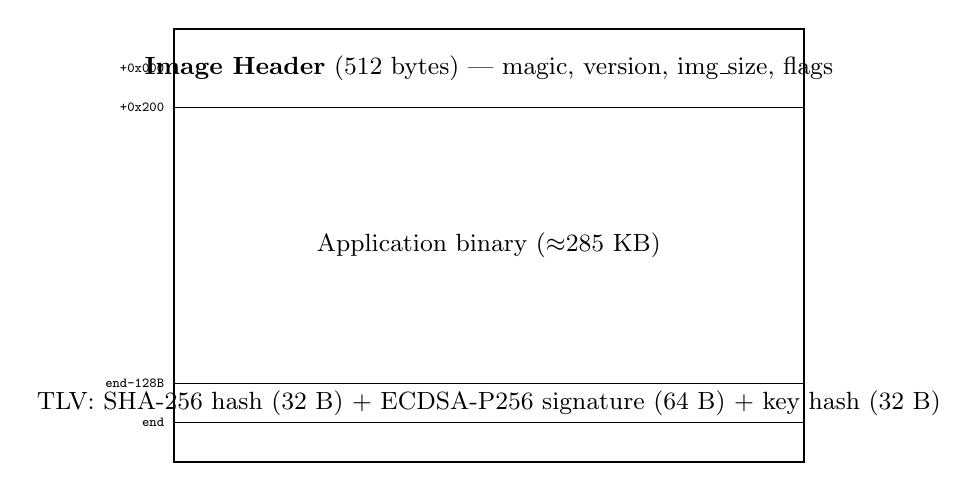
\begin{tikzpicture}[font=\small]
  \draw[thick] (0,0) rectangle (8,5.5);
  \draw (0,4.5) -- (8,4.5);  % header line
  \draw (0,1.0) -- (8,1.0);  % TLV info line
  \draw (0,0.5) -- (8,0.5);

  \node at (4, 5.0) {\textbf{Image Header} (512 bytes) — magic, version, img\_size, flags};
  \node at (4, 2.75) {Application binary ($\approx$285~KB)};
  \node at (4, 0.75) {TLV: SHA-256 hash (32~B) + ECDSA-P256 signature (64~B) + key hash (32~B)};
  \node[font=\tiny,left] at (0,5.0) {\texttt{+0x000}};
  \node[font=\tiny,left] at (0,4.5) {\texttt{+0x200}};
  \node[font=\tiny,left] at (0,1.0) {\texttt{end-128B}};
  \node[font=\tiny,left] at (0,0.5) {\texttt{end}};
\end{tikzpicture}
\end{center}

\subsection{Key DTS Lesson: MCUboot \texttt{chosen} Override}

The board DTS (\texttt{nucleo\_h753zi.dts}) sets \texttt{zephyr,code-partition = \&slot0\_partition}
in its chosen node. Without an explicit override, MCUboot links itself to slot0 (0x08040000)
instead of \texttt{boot\_partition} (0x08000000) — meaning the app flash writes overwrite the bootloader.

The fix, in \texttt{sysbuild/mcuboot.overlay}:
\begin{lstlisting}[language=C, caption={MCUboot chosen override}]
/ {
    chosen {
        zephyr,code-partition = &boot_partition;
    };
};
\end{lstlisting}

% ═════════════════════════════════════════════════════════════════════════════
\section{Phase 3b — OTA Firmware Update}

\subsection{API Endpoints}

\begin{center}
\begin{tabular}{@{}lllp{5cm}@{}}
\toprule
\textbf{Route} & \textbf{Method} & \textbf{Auth} & \textbf{Purpose} \\
\midrule
\texttt{/ota}           & GET  & Session or Bearer & Browser upload page with progress bar \\
\texttt{/api/firmware}  & POST & Session or Bearer & Stream binary to slot1, arm upgrade \\
\texttt{/api/reboot}    & POST & Session or Bearer & Cold reboot into MCUboot swap \\
\bottomrule
\end{tabular}
\end{center}

\subsection{Upload Protocol}

\begin{lstlisting}[language=bash, caption={OTA via curl}]
TOKEN="<64-char hex from http_auth.hpp>"

# Upload firmware
curl -X POST http://192.168.1.80/api/firmware       \
     -H "Authorization: Bearer $TOKEN"              \
     -H "Content-Type: application/octet-stream"    \
     --data-binary @build/zephyr/zephyr/zephyr.signed.bin
# Response: {"status":"ok","bytes":292772}

# Trigger swap
curl -X POST http://192.168.1.80/api/reboot         \
     -H "Authorization: Bearer $TOKEN"
# Response: {"status":"rebooting"}
\end{lstlisting}

\subsection{OTA State Machine}

\begin{center}
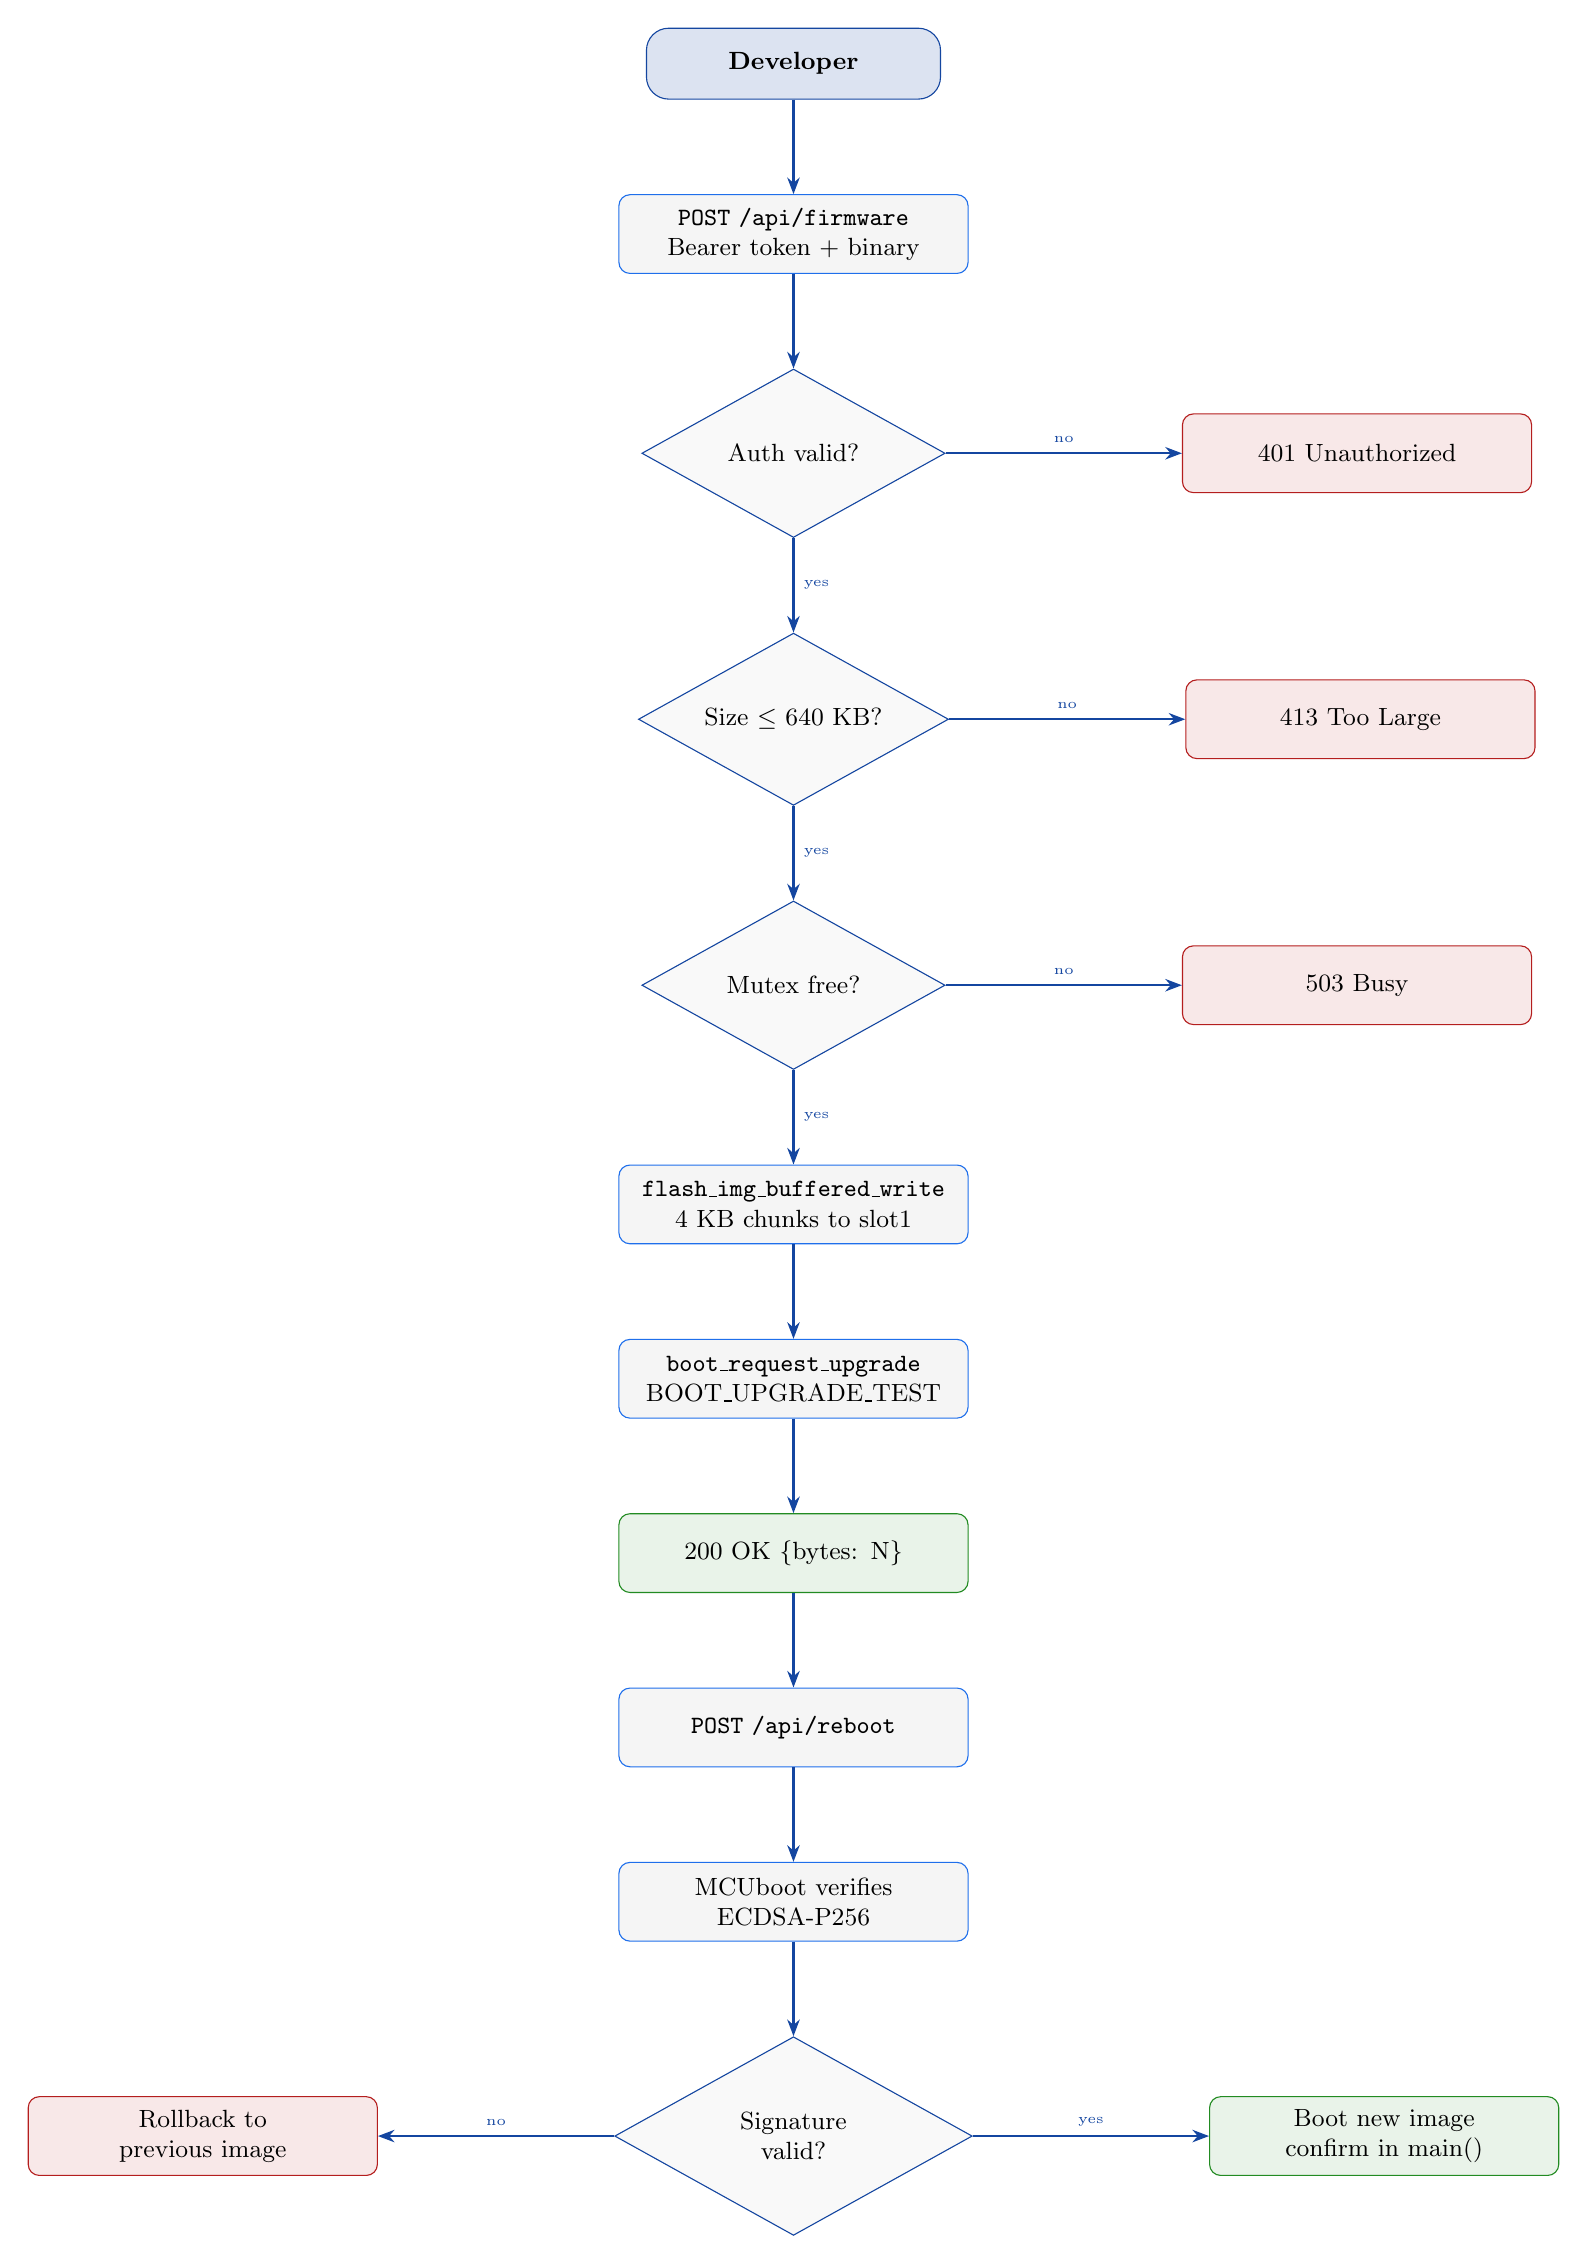
\begin{tikzpicture}[node distance=1.2cm, every node/.style={font=\small}]
  \node[term]                       (dev)   {Developer};
  \node[block, below=of dev]        (post)  {\texttt{POST /api/firmware}\\Bearer token + binary};
  \node[decision, below=of post]    (auth)  {Auth valid?};
  \node[errblock, right=3cm of auth](r401)  {401 Unauthorized};
  \node[decision, below=of auth]    (size)  {Size $\leq$ 640~KB?};
  \node[errblock, right=3cm of size](r413)  {413 Too Large};
  \node[decision, below=of size]    (mtx)   {Mutex free?};
  \node[errblock, right=3cm of mtx] (r503)  {503 Busy};
  \node[block, below=of mtx]        (write) {\texttt{flash\_img\_buffered\_write}\\4~KB chunks to slot1};
  \node[block, below=of write]      (arm)   {\texttt{boot\_request\_upgrade}\\BOOT\_UPGRADE\_TEST};
  \node[okblock, below=of arm]      (r200)  {200 OK \{bytes: N\}};
  \node[block, below=of r200]       (rb)    {\texttt{POST /api/reboot}};
  \node[block, below=of rb]         (boot)  {MCUboot verifies\\ECDSA-P256};
  \node[decision, below=of boot]    (sig)   {Signature\\valid?};
  \node[okblock, right=3cm of sig]  (ok)    {Boot new image\\confirm in main()};
  \node[errblock, left=3cm of sig]  (rl)    {Rollback to\\previous image};

  \draw[arr] (dev)   -- (post);
  \draw[arr] (post)  -- (auth);
  \draw[arr] (auth)  -- node[above,font=\tiny]{no}  (r401);
  \draw[arr] (auth)  -- node[right,font=\tiny]{yes} (size);
  \draw[arr] (size)  -- node[above,font=\tiny]{no}  (r413);
  \draw[arr] (size)  -- node[right,font=\tiny]{yes} (mtx);
  \draw[arr] (mtx)   -- node[above,font=\tiny]{no}  (r503);
  \draw[arr] (mtx)   -- node[right,font=\tiny]{yes} (write);
  \draw[arr] (write) -- (arm);
  \draw[arr] (arm)   -- (r200);
  \draw[arr] (r200)  -- (rb);
  \draw[arr] (rb)    -- (boot);
  \draw[arr] (boot)  -- (sig);
  \draw[arr] (sig)   -- node[above,font=\tiny]{yes} (ok);
  \draw[arr] (sig)   -- node[above,font=\tiny]{no}  (rl);
\end{tikzpicture}
\end{center}

\subsection{Rollback Safety}

MCUboot's \texttt{BOOT\_UPGRADE\_TEST} mode ensures the new image must explicitly confirm
itself within one boot cycle or MCUboot restores the previous image:

\begin{enumerate}[nosep]
\item Upload sets swap magic in slot1 trailer; \texttt{image\_ok = 0}.
\item On next boot, MCUboot swaps slot1 $\to$ slot0 and boots new image.
\item \texttt{boot\_write\_img\_confirmed()} in \texttt{main.cpp} writes \texttt{image\_ok = 1}.
\item On the \emph{next} boot, MCUboot sees \texttt{image\_ok = 1} and does not swap back.
\item If the new image crashes before reaching \texttt{main()}, the next boot finds
      \texttt{image\_ok = 0} and MCUboot rolls back automatically.
\end{enumerate}

\subsection{Implementation Notes}

\begin{itemize}[nosep]
\item \texttt{CONFIG\_IMG\_ERASE\_PROGRESSIVELY=y}: sectors are erased on the first write
      to them — no full pre-erase of slot1 required before upload.
\item \texttt{K\_MUTEX\_DEFINE(g\_ota\_mutex)}: prevents concurrent uploads from corrupting
      the flash write context.
\item Static 4~KB receive buffer (\texttt{s\_rx\_buf}): prevents stack overflow on the
      HTTP server thread during large uploads.
\item \texttt{handle\_api\_reboot()} calls \texttt{zsock\_close(fd)} then waits 200~ms
      before \texttt{sys\_reboot(SYS\_REBOOT\_COLD)} to allow TCP to flush the response.
\end{itemize}

% ═════════════════════════════════════════════════════════════════════════════
\section{Threat Model}

\begin{longtable}{@{}p{4cm}p{3.5cm}p{5cm}@{}}
\toprule
\textbf{Threat} & \textbf{Control} & \textbf{Residual Risk} \\
\midrule
\endhead
Unauthenticated HTTP command & Bearer token (256-bit) & Token in plaintext on LAN (no TLS yet) \\
Session hijack & 1-hour TTL, 4-slot table & Cookie in plaintext (no TLS yet) \\
Rogue firmware via OTA & ECDSA-P256 signature required & Attacker needs private key \\
Bricked device from bad OTA & Test-mode rollback & None — automatic recovery \\
Firmware extraction via SWD & (Phase 4) RDP Level 1 & Currently readable \\
Firmware hang / DoS & IWDG 1~s timeout → reboot & None for single-fault \\
Power-loss during OTA swap & MCUboot scratch area + test-mode & None — swap is resumable \\
Replay of captured token & Bearer token static (no nonce) & Mitigated by HTTPS (planned) \\
\bottomrule
\end{longtable}

% ═════════════════════════════════════════════════════════════════════════════
\section{Phase 4 Preview — RDP Level 1}

\textbf{Not yet applied.} Will be set as the absolute last production step.

Setting the \texttt{RDP} option byte to \texttt{0xBB} activates Read Protection Level~1:

\begin{itemize}[nosep]
\item SWD/JTAG can halt the CPU and program flash — development and OTA workflow unchanged.
\item SWD/JTAG \textbf{cannot read back} flash contents — firmware extraction is blocked.
\item The ROM UART bootloader can write new firmware but cannot read back.
\item Downgrading to Level~0 triggers a \textbf{full mass erase} — all firmware is wiped.
      After mass erase, the board must be re-flashed from scratch via JTAG or ROM UART bootloader.
\end{itemize}

After RDP Level~1, OTA (Phase~3b) becomes the primary in-field update mechanism.

% ═════════════════════════════════════════════════════════════════════════════
\section{Kconfig and File Reference}

\subsection{Key Kconfig Options}

\begin{center}
\begin{tabular}{@{}lll@{}}
\toprule
\textbf{Option} & \textbf{Value} & \textbf{Purpose} \\
\midrule
\texttt{CONFIG\_BOOTLOADER\_MCUBOOT}         & \texttt{y}   & App linked to slot0, adds image header \\
\texttt{CONFIG\_IMG\_MANAGER}                & \texttt{y}   & OTA and confirmation APIs \\
\texttt{CONFIG\_FLASH\_MAP}                  & \texttt{y}   & Flash area abstraction \\
\texttt{CONFIG\_STREAM\_FLASH}               & \texttt{y}   & Streaming write for OTA \\
\texttt{CONFIG\_IMG\_ERASE\_PROGRESSIVELY}   & \texttt{y}   & Erase on-demand during write \\
\texttt{CONFIG\_WATCHDOG}                    & \texttt{y}   & Zephyr WDT driver \\
\texttt{CONFIG\_BOOT\_SIGNATURE\_TYPE\_ECDSA\_P256} & \texttt{y} & MCUboot signature algorithm \\
\texttt{CONFIG\_BOOT\_MAX\_IMG\_SECTORS}     & \texttt{512} & Max sectors per slot \\
\bottomrule
\end{tabular}
\end{center}

\subsection{Critical Files}

\begin{center}
\begin{tabular}{@{}ll@{}}
\toprule
\textbf{File} & \textbf{Purpose} \\
\midrule
\texttt{zephyr/app.overlay}                   & Flash partition layout for app \\
\texttt{zephyr/sysbuild/mcuboot.overlay}      & MCUboot partition layout + chosen override \\
\texttt{zephyr/sysbuild/mcuboot.conf}         & MCUboot Kconfig (ECDSA-P256) \\
\texttt{zephyr/sysbuild.conf}                 & \texttt{SB\_CONFIG\_BOOTLOADER\_MCUBOOT=y} \\
\texttt{zephyr/CMakeLists.txt}                & \texttt{MCUBOOT\_SIGNING\_KEY\_FILE} \\
\texttt{zephyr/mcuboot\_signing\_key.pem}     & ECDSA-P256 private key (gitignored) \\
\texttt{zephyr/src/main.cpp}                  & \texttt{boot\_write\_img\_confirmed()} \\
\texttt{zephyr/src/http/http\_ota.cpp}        & OTA upload, page, reboot handlers \\
\texttt{zephyr/src/http/http\_server.cpp}     & Route table (includes OTA routes) \\
\texttt{zephyr/src/watchdog/watchdog\_thread.cpp} & IWDG kicks + semaphore monitoring \\
\bottomrule
\end{tabular}
\end{center}

\end{document}
